\documentclass{article}
\usepackage[utf8]{inputenc}
\usepackage{amsmath}
\usepackage{indentfirst}
\usepackage{graphicx,caption}
\usepackage[a4paper, margin=1in]{geometry}
\linespread{1.15}
\usepackage{empheq}
\usepackage[most]{tcolorbox}
\usepackage[margin=3cm]{caption}
\usepackage{siunitx}

\usepackage{xcolor,sectsty}
\definecolor{astral}{RGB}{46,116,181}
\subsectionfont{\color{astral}}
\sectionfont{\color{astral}}

\title{
\includegraphics[width=0.1\textwidth]{ufallogo.png} \\
\Huge{\color{astral}\textbf{Propriedades Eletromagnéticas da Matéria}}}
\author{Paulo Brandão}
\date{Maio de 2017}

\newtcbox{\mymath}[1][]{%
    nobeforeafter, math upper, tcbox raise base,
    enhanced, colframe=blue!30!black,
    colback=blue!30, boxrule=1pt,
    #1}

\begin{document}

\maketitle

\section{Introdução}

O estudo da matéria e suas propriedades térmicas, mecânicas e eletromagnéticas é descrito de forma geral pela importante área de pesquisa conhecida como \textbf{física da matéria condensada}. Esse é o campo da física que lida com as propriedades físicas microscópicas e macroscópicas da matéria e sua resposta à estímulos externos. Essa área de pesquisa varia desde aplicações de engenharia do dia-a-dia até tópicos que beiram a teoria das cordas da física de partículas! O ponto em comum de todos esses fenômenos é que eles são relacionados com a maneira na qual os constituintes da matéria interagem entre eles e com estímulos externos. Uma subárea muito importante da matéria condensada lida com sólidos, isto é, com materiais que possuem uma rede cristalina. Esse campo é chamado de \textbf{física do estado sólido} e seu objetivo é compreender as propriedades mecânicas, térmicas, eletromagnéticas, etc, de compostos sólidos. É fácil perceber que o estudo das propriedades eletromagnéticas da matéria, num contexto geral, é extremamente amplo, complexo e permeado por diferentes tipos de formalismos que misturam diferentes pontos de vista quânticos e clássicos. Se torna impossível, em uma única aula, tratar de todos os sistemas materiais e suas interações com campos eletromagnéticos em sua generalidade completa. Além disso, nem sempre o formalismo que é utilizado para estudar a resposta da matéria num determinado domínio de frequências é útil em outras faixas do espectro eletromagnético. Em alguns casos, uma análise macroscópica clássica é suficiente para explicar o fenômeno observado enquanto que em outras situações a teoria quântica deve ser empregada para se obter uma descrição completa do efeito. Dessa forma, nesta aula, iremos tratar apenas do formalismo clássico da interação radiação-matéria descrito pelas equações de Maxwell. A pergunta que tentaremos responder ao longo da aula será: dado um material, como podemos descrever sua interação com o campo eletromagnético? 

Começamos a discussão na seção 2 introduzindo o formalismo necessário para a descrição da interação radiação-matéria de um ponto de vista clássico através do uso das equações de Maxwell. Uma aproximação linear será discutida e introduzimos a importante quantidade chamada de função dielétrica que irá ser estudada no decorrer de toda a aula. A seção 3 se concentra na resposta linear e nos problemas de causalidade impostos pelas relações de Kramers-Kroning. Uma discussão importante sobre dispersão temporal e espacial também é considerada. Na seção 4 estudaremos o caso particular da dependência da função dielétrica com a frequência do campo externo e derivaremos uma relação muito importante para a parte real da função dielétrica. A seção 5 descreve brevemente o comportamento de uma onda eletromagnética quando a mesma se propaga num meio dispersivo. Na seção 6 discutiremos a origem física das ressonâncias existentes num espectro de absorção, caracterizado pela parte imaginária da função dielétrica. Apenas trataremos a contribuição eletrônica da função dielétrica. Concluímos a aula na seção 7 com uma discussão breve sobre as outras formas de ressonâncias existentes nos materiais.


\section{Equações de Maxwell num Meio Dielétrico}

Estaremos interessados nessa aula em descrever a interação entre radiação eletromagnética e a matéria de um ponto de vista macroscópico. Iremos sempre assumir que a variação do campo elétrico através do material estudado envolve escalas de distâncias muito maiores que o tamanho das moléculas ou átomos que formam o material. Na porção visível do espectro eletromagnético, por exemplo, o comprimento de onda é da ordem de $10^{-5}$ cm enquanto que o tamanho de uma ligação molecular típica ou de uma constante de rede cristalina é da ordem de $10^{-8}$ cm. A descrição clássica macroscópica da interação da matéria com campos eletromagnéticos é obtida, nesse contexto, através das equações de Maxwell (em unidades SI):
\begin{equation}
    \nabla\cdot\mathbf{D} = 0,
\end{equation}
\begin{equation}
    \nabla\cdot\mathbf{B} = 0,
\end{equation}
\begin{equation}
    \nabla\times\mathbf{H} = \frac{\partial \mathbf{D}}{\partial t}
\end{equation}
\begin{equation}
    \nabla\times\mathbf{E} = -\frac{\partial \mathbf{B}}{\partial t},
\end{equation}
onde $\mathbf{E}$ é o campo elétrico, $\mathbf{D}$ o vetor deslocamento elétrico, $\mathbf{H}$ o campo magnético e $\mathbf{B}$ o vetor indução magnética. Assumi que o sistema considerado não possui cargas nem correntes livres. Para proceder, precisamos das relações entre os vários campos que entram nas equações de Maxwell. No limite de interesse, podemos escrever
\begin{equation}
    \mathbf{D} = \varepsilon_0 \mathbf{E} + \mathbf{P}
\end{equation}
e
\begin{equation}
    \mathbf{B} = \mu_0( \mathbf{H} + \mathbf{M} ),
\end{equation}
onde $\mathbf{P}$ e $\mathbf{M}$ são o momento de dipolo elétrico por unidade de volume e o momento magnético por unidade de volume, respectivamente \footnote{Não chamarei $\mathbf{P}$ de polarização como alguns livros fazem porque a palavra polarização também pode designar direção do campo elétrico, que possui um sentido completamente diferente do que estamos discutindo aqui.}. Iremos considerar apenas materiais não-magnéticos, isto é, materiais tal que $\mathbf{M} = 0$ que implica a relação linear $\mathbf{B} = \mu_0 \mathbf{H}$. Para continuar nossa análise, precisamos estabelecer a relação entre o campo elétrico $\mathbf{E}$ e a densidade de dipolo elétrico $\mathbf{P}$ do material. Em princípio, seria necessária uma teoria microscópica para relacionar o campo elétrico $\mathbf{E}$ (macroscópico) com os dipolos elétricos (microscópicos) do material. Porém, é possível desenvolver uma análise fenomenológica desses parâmetros, como iremos demonstrar agora.

Os campos elétricos mais fortes encontrados em laboratórios usuais são da ordem de $10^8$ V/m. Um elétron ligado à um átomo ou molécula, ou movendo-se por um sólido ou líquido, sente a presença de campos elétricos da ordem de $10^{11}$ V/m, como pode ser facilmente verificado a partir de estimativas de ordem de grandeza. Os campos de laboratório são portanto pequenos comparados aos campos sentidos pelos elétrons de forma que podemos expandir a densidade de dipolo elétrico numa série de Taylor em torno do campo elétrico:
\begin{equation}
    P_{\alpha}(\mathbf{r},t) = P^{(0)}_\alpha + \varepsilon_0\sum_{\beta}\left( \frac{\partial P_\alpha}{\partial E_\beta} \right)_0 E_\beta + \frac{\varepsilon_0}{2!}\sum_{\beta\gamma}\left( \frac{\partial^2 P_\alpha}{\partial E_\beta \partial E_\gamma} \right)_0 E_\beta E_\gamma + ...,
    \label{eq7}
\end{equation}
onde $\alpha$, $\beta$, $\gamma$, são índices que tomam valores de $x$, $y$ e $z$. Assumi na Equação \eqref{eq7} que a densidade de dipolo elétrico numa posição $\mathbf{r}$ e no tempo $t$ depende do campo na mesma posição $\mathbf{r}$ e no mesmo tempo $t$. Entretanto, essa suposição é incorreta de um ponto de vista fundamental que tem uma relação com a causalidade! Iremos ver mais adiante como podemos contornar esse obstáculo para uma análise mais precisa. Porém, em muitos casos a relação acima é uma boa aproximação.

O termo $P_\alpha^{(0)}$ é nulo na grande maioria dos materiais comuns. Ele representa uma densidade de dipolo elétrico na ausência de qualquer outro campo elétrico externo. A situação usual é que a presença de dipolos elétricos por unidade de volume num material aparece somente quando os mesmos são induzidos pelo campo externo. Materiais que precisam do termo $P_\alpha^{(0)}$ para uma descrição completa da densidade de dipolos são chamados de \textbf{ferroelétricos}. Eles são os análogos elétricos dos materiais mais comuns chamados de ferromagnéticos. Assim como os ferromagnéticos, os ferroelétricos podem perder sua densidade de dipolos elétricos caso uma certa temperatura seja atingida, conhecida como temperatura de Curie. A origem da densidade espontânea de dipolos elétricos num ferroelétrico está no deslocamento de um íon de um alto ponto de simetria para um ponto de simetria mais baixa quando sua temperatura diminui. Esse deslocamento do íon dá origem ao dipolo elétrico e esse é um fenômeno coletivo onde todos os íons irão fornecer uma quantidade de dipolos por volume. Esses materiais respondem fortemente aos campos elétricos estáticos ou de frequências muito baixas. Num ferroelétrico, a densidade de dipolo elétrico, $\mathbf{P}^{(0)}$, na ausência de um campo elétrico externo, é independente do tempo mas pode variar com a posição. O campo elétrico macroscópico $\mathbf{E}^{0}(\mathbf{r})$ criado pelo material obedece as equações da eletrostática
\begin{equation}
    \nabla\times\mathbf{E}^{(0)} = 0
\end{equation}
e
\begin{equation}
    \nabla\cdot\mathbf{E}^{(0)} = -\nabla\cdot\mathbf{P}^{(0)} = \rho_b,
\end{equation}
onde $\rho_b = -\nabla\cdot\mathbf{P}^{(0)}$ se torna a densidade de carga efetiva presente na equação de Poisson.

Estaremos interessados em campos elétricos dependentes do tempo criados pelo material quando o mesmo interage com radiação externa, um laser por exemplo. Assim, iremos desprezar a contribuição da densidade de momento de dipolo estática. Podemos reescrever a Equação \eqref{eq7} na forma
\begin{equation}
    P_\alpha (\mathbf{r},t) = \varepsilon_0\sum_{\beta} \chi^{(1)}_{\alpha\beta} E_\beta + \varepsilon_0\sum_{\beta\gamma}\chi^{(2)}_{\alpha\beta\gamma} E_\beta E_\gamma + ...,
\end{equation}
onde $\chi^{(1)}_{\alpha\beta}$ e $\chi^{(2)}_{\alpha\beta\gamma}$ são as susceptibilidades de primeira e segunda ordem. Claramente a expansão continua com a introdução de susceptibilidades de ordens três, quatro, etc. As susceptibilidades são tensores em geral. Assim, $\chi^{(1)}_{\alpha\beta}$ é um tensor de segunda ordem. Para um material isotrópico como um gás, um líquido ou um cristal com simetria cúbica: $\chi^{(1)}_{\alpha\beta} = \chi^{(1)} \delta_{\alpha\beta}$. Ou seja, o tensor de primeira ordem se torna diagonal.

Podemos separar a expressão da densidade de dipolos elétricos em duas contribuições, uma linear e outra não-linear no campo:
\begin{equation}
    P_\alpha (\mathbf{r},t) = P^{\text{L}}_\alpha (\mathbf{r},t) + P^{\text{NL}}_\alpha (\mathbf{r},t),
\end{equation}
onde
\begin{equation}
P^{\text{L}}_\alpha (\mathbf{r},t) = \varepsilon_0\sum_{\beta} \chi^{(1)}_{\alpha\beta} E_\beta
\label{eq12}
\end{equation}
e
\begin{equation}
P^{\text{NL}}_\alpha (\mathbf{r},t) = \varepsilon_0\sum_{\beta\gamma}\chi^{(2)}_{\alpha\beta\gamma} E_\beta E_\gamma + ... .
\end{equation}
Se considerarmos apenas $P^{\text{L}}_\alpha (\mathbf{r},t)$ na análise, e combinarmos isso com as equações de Maxwell então obtemos uma descrição da propagação de ondas eletromagnéticas num meio, de natureza possivelmente cristalina, descrita pelo tensor de susceptibilidade elétrica $\chi_{\alpha\beta}$. De fato:
\begin{equation}
\begin{split}
    D_{\alpha}(\mathbf{r},t) & = \varepsilon_{0} E_\alpha + P^{\text{L}}_\alpha \\
    & = \varepsilon_{0} E_\alpha + \varepsilon_0\sum_{\beta} \chi^{(1)}_{\alpha\beta} E_\beta \\
    & = \varepsilon_0\sum_{\beta}\delta_{\alpha\beta}E_\beta + \varepsilon_0\sum_{\beta} \chi^{(1)}_{\alpha\beta} E_\beta \\
    & = \varepsilon_0 \sum_{\beta}\varepsilon_{\alpha\beta}E_\beta
\end{split}
\end{equation}
onde $\varepsilon_{\alpha\beta} = \delta_{\alpha\beta} + \chi_{\alpha\beta}^{(1)}$ é o tensor dielétrico do material. O cálculo das susceptibilidades não-lineares requer uma teoria microscópica apropriada para o material em questão. É possível escrever expressões formais para essas quantidades, porém, elas são incrivelmente complicadas e não muito úteis para tratar de uma forma geral. Iremos tratar os coeficientes na expansão da densidade de dipolo elétrico simplesmente como grandezas fenomenológicas.

Existe um outro tratamento que pode ser utilizado para obter expressões para as susceptibilidades lineares e não-lineares partindo de um ponto de vista microscópico que modela a estrutura atômica ou molecular de maneira explícita. Assim, a densidade de momento de dipolo elétrico, $\mathbf{P}$, é relacionada com o momento de dipolo elétrico $\mathbf{p}$ de cada elemento constituinte. Nesse caso, o campo elétrico que entra na expansão não é o campo macroscópico que utilizamos na discussão acima mas sim o campo microscópico, formado pela soma do campo externo com o campo criado por todos os outros dipolos. Claramente, o campo microscópico pode ser bastante diferente do campo macroscópico. Entretanto, é sempre o caso de que o campo local é sempre proporcional ao campo macroscópico; uma consequência disso é que a densidade de momento de dipolo sempre pode ser expandida em potências do campo macroscópico, como fizemos anteriormente.

\section{Resposta Dielétrica Linear da Matéria}

Estaremos interessados inicialmente na resposta linear da matéria, isto é, apenas na contribuição do termo \eqref{eq12}. A natureza tensorial da susceptibilidade elétrica linear pode ser desprezada numa primeira análise para facilitar a introdução de alguns conceitos novos. Dessa forma, tomamos $\chi_{\alpha\beta}^{(1)} = \delta_{\alpha\beta}\chi$, de tal forma que a densidade dipolo elétrico é dada por
\begin{equation}
    P_{\alpha} (\mathbf{r},t) = \varepsilon_0 \chi E_{\alpha} (\mathbf{r},t).
\label{eq15}
\end{equation}
A relação entre a densidade de dipolo elétrico e o campo elétrico macroscópico descrita pela Equação \eqref{eq15} é claramente uma aproximação no sentido de que o surgimento de uma densidade de dipolo elétrico no tempo $t$ não pode ter aparecido no mesmo tempo $t$ em que o campo interagiu com a matéria. Esperamos que \textit{após um certo tempo} de interação das moléculas ou átomos com o campo é que comecem a aparecer densidades de dipolo elétrico. A relação \eqref{eq15} deve ser modificada para incluir a defasagem de tempo entre a aplicação do campo elétrico e a criação da densidade de dipolos. Isto é feito através da generalização da equação \eqref{eq15}:
\begin{empheq}[box=\tcbhighmath]{equation}
    P_\alpha (\mathbf{r},t) = \varepsilon_0 \int\displaylimits_{+\infty}^{-\infty} dt' R(t-t')E_\alpha (\mathbf{r},t'),
    \label{eq16}
\end{empheq}
onde $R(t')$ é a função resposta do sistema. A Equação \eqref{eq16} expressa uma \textit{convolução temporal} entre a função resposta e o campo elétrico na posição fixa $\mathbf{r}$. Matemáticos escrevem essa relação como $P_{\alpha}(\mathbf{r},t) = \varepsilon_0 R(t)\star E_\alpha(\mathbf{r},t)$. A função $R(t')$ deve satisfazer a relação $R = 0$ para $t'<0$ para não violar a causalidade, como iremos detalhar agora.

Suponha que o campo elétrico $E_\alpha (t')$ atua numa posição $\mathbf{r}$ (não mostrada) dentro do material, como ilustra a Figura 1, e que o mesmo responde através da criação da densidade de dipolo elétrico $P_{\alpha}(t')$. A função resposta $R(t')$ é mostrada na Figura 1. A polarização é dada pela área do gráfico (para cada tempo $t$) do produto entre $R(t-t')$ e $E(t')$. Fica claro assim que a densidade de dipolo elétrico varia no tempo de uma forma bem diferente do que seria esperado através da relação $P_\alpha(t) = \varepsilon_0 \chi E_\alpha (t)$. A relação \eqref{eq15} é um caso particular da relação \eqref{eq16} quando o campo elétrico varia de uma maneira muito lenta comparada à variação da função resposta $R(t')$. Nesse caso, é possível remover o campo elétrico da integral na relação \eqref{eq16} e, através da definição
\begin{equation}
    \chi = \int\displaylimits_{-\infty}^{+\infty} R(t-t') dt',
\end{equation}
podemos retomar \eqref{eq15}. Note que a integral acima não depende de $t$ e, portanto, $\chi$ é uma quantidade independente do tempo.

\begin{figure}[ht]
\centering
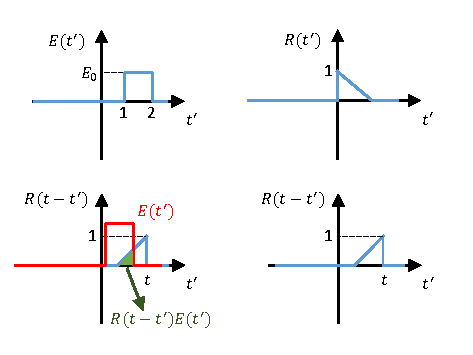
\includegraphics[width=8cm]{fig1.pdf}
\caption{Ilustração da resposta do meio em termos da convolução entre o campo elétrico representado por um pulso quadrado e a função resposta dada por uma reta com coeficiente angular negativo. A convolução, para cada tempo $t$, é dada pela área verde no gráfico inferior à esquerda.}
\end{figure}

A densidade de dipolos elétricos induzida numa posição $\mathbf{r}$ dentro do material vai depender também dos dipolos induzidos nas vizinhanças desse ponto. Assim, uma relação direta entre a posição da densidade de dipolos e a posição do campo elétrico também deve ser incluída na função resposta. Podemos escrever a relação mais geral
\begin{empheq}[box=\tcbhighmath]{equation}
    P_{\alpha}(\mathbf{r},t) = \varepsilon_0 \sum_{\beta}\int dt' \int d^{3}r' R_{\alpha\beta}(\mathbf{r}-\mathbf{r}',t-t')E_{\beta}(\mathbf{r}',t').
    \label{eq18}
\end{empheq}
Se o material é de natureza homogênea, então a resposta dielétrica $R$ depende apenas da diferença $\mathbf{r}-\mathbf{r}'$. Se existe, por exemplo, variações na densidade ou na decomposição do material, uma descrição mais complexa deve ser empregada. Se o campo elétrico exibe uma variação lenta no espaço e no tempo, podemos remover o campo da integral e definir
\begin{equation}
    \chi_{\alpha\beta} = \int dt' d^{3}r' R_{\alpha\beta}(\mathbf{r}-\mathbf{r}',t-t')
\end{equation}
para obter o caso particular onde a resposta do meio é aproximadamente instantânea com o campo elétrico.

As expressões para a densidade de dipolos elétricos é bastante complicada nas variáveis ($\mathbf{r},t$). É possível simplificar a análise escrevendo o campo elétrico no espaço das frequências espaciais e temporais $(\mathbf{k},\omega)$. Suponha que o campo elétrico é escrito na base de ondas planas:
\begin{equation}
    E_{\beta} (\mathbf{r},t) = \int \frac{d^3 k d\omega}{(2\pi)^4} E_{\beta}(\mathbf{k},\omega)e^{i\mathbf{k}\cdot\mathbf{r}-i\omega t}.
\end{equation}
Substituindo o campo na expressão \eqref{eq18},
\begin{equation}
\begin{split}
P_{\alpha}(\mathbf{r},t) & = \varepsilon_0 \sum_{\beta}\int dt' \int d^{3}r' R_{\alpha\beta}(\mathbf{r}-\mathbf{r}',t-t')\int \frac{d^3 k d\omega}{(2\pi)^4} E_{\beta}(\mathbf{k},\omega)e^{i\mathbf{k}\cdot\mathbf{r}'-i\omega t'}\\ 
&= \frac{\varepsilon_0}{(2\pi)^4}\int d^3 k d\omega \sum_{\beta}\int dt' \int d^{3}r' R_{\alpha\beta}(\mathbf{r}-\mathbf{r}',t-t') e^{i\mathbf{k}\cdot\mathbf{r}'-i\omega t'}E_{\beta}(\mathbf{k},\omega) \\
&= \frac{\varepsilon_0}{(2\pi)^4}\int d^3 k d\omega \sum_{\beta}\int dT \int d^{3}u R_{\alpha\beta}(\mathbf{u},T) e^{-i\mathbf{k}\cdot\mathbf{u}+i\omega T}e^{i\mathbf{k}\cdot\mathbf{r}-i\omega t}E_{\beta}(\mathbf{k},\omega) \\
&= \frac{\varepsilon_0}{(2\pi)^4}\int d^3 k d\omega \sum_{\beta}\chi_{\alpha\beta}(\mathbf{k},\omega)e^{i\mathbf{k}\cdot\mathbf{r}-i\omega t}E_{\beta}(\mathbf{k},\omega) \\
&= \int \frac{d^3 k d\omega}{(2\pi)^4} P_{\alpha}(\mathbf{k},\omega)e^{i\mathbf{k}\cdot\mathbf{r}-i\omega t},
\end{split}
\end{equation}
onde
\begin{equation}
    P_\alpha (\mathbf{k},\omega) = \varepsilon_0 \sum_\beta \chi_{\alpha\beta}(\mathbf{k},\omega)E_\beta (\mathbf{k},\omega)
\end{equation}
e
\begin{equation}
    \chi_{\alpha\beta}(\mathbf{k},\omega) = \int dt \int d^{3}r R_{\alpha\beta}(\mathbf{r},t) e^{-i\mathbf{k}\cdot\mathbf{r}+i\omega t}.
\end{equation}
É mais comum na teoria dielétrica linear considerar a relação entre o vetor deslocamento elétrico $\mathbf{D}$ e o campo elétrico $\mathbf{E}$. No espaço das frequências $(\mathbf{k},\omega)$:
\begin{equation}
    D_\alpha (\mathbf{k},\omega) = \varepsilon_0 \sum_\beta \varepsilon_{\alpha\beta}(\mathbf{k},\omega)E_\beta (\mathbf{k},\omega)
\end{equation}
donde segue que
\begin{empheq}[box=\tcbhighmath]{equation}
    \varepsilon_{\alpha\beta}(\mathbf{k},\omega) = \delta_{\alpha\beta} + \chi_{\alpha\beta}(\mathbf{k},\omega)
\end{empheq}
é o tensor dielétrico do material. A variação da resposta dielétrica com a frequência temporal $\omega$ é um fenômeno bastante conhecido e estudado chamado de dispersão temporal. A grande maioria dos livros-texto, entretanto, não enfatizam muito o caráter temporal da resposta dielétrica como apresentei aqui. A dependência da resposta dielétrica na frequência espacial $\mathbf{k}$, por outro lado, é discutida muito pouco. No regime óptico, o comprimento de onda da radiação eletromagnética é da ordem de 5000 \si{\angstrom}, ou seja, aproximadamente mil vezes maior que o comprimento das ligações moleculares ou constante de rede (2-3 \si{\angstrom}). Nessas circunstâncias, é válido aproximar $\mathbf{k}\rightarrow 0$ e trabalhar apenas com a dependência em $\omega$ do tensor dielétrico: $\varepsilon_{\alpha\beta}(\mathbf{k}\rightarrow 0,\omega) = \varepsilon_{\alpha\beta}(\omega)$. 


\section{Dependência da Frequência no Tensor Dielétrico}

Vamos assumir que estamos interessados na propagação da radiação eletromagnética num meio isotrópico e sem dispersão espacial. A relação entre o vetor deslocamento elétrico e o campo elétrico é dada por
\begin{equation}
\begin{split}
    D_\alpha (\mathbf{r},t) &= \varepsilon_0 \int\displaylimits_{-\infty}^{+\infty}dt' R(t-t')E_\alpha (\mathbf{r},t') \\
    &= \varepsilon_0 \int\displaylimits_{-\infty}^{+\infty}dt' R(t-t')\int\displaylimits_{-\infty}^{+\infty} E_\alpha (\mathbf{r},\omega)e^{-i\omega t'}d\omega \\
    &= \varepsilon_0 \int\displaylimits_{-\infty}^{+\infty}dt''  \int\displaylimits_{-\infty}^{+\infty}d\omega R(t'')e^{-i\omega(t-t'')} E_\alpha (\mathbf{r},\omega) \\
    &= \varepsilon_0 \int\displaylimits_{-\infty}^{+\infty} d\omega \int\displaylimits_{-\infty}^{+\infty} R(t'')e^{i\omega t''}dt'' E_\alpha (\mathbf{r},\omega) e^{-i\omega t} \\
    &= \varepsilon_0 \int\displaylimits_{-\infty}^{+\infty} d\omega \varepsilon(\omega) E_\alpha (\mathbf{r},\omega) e^{-i\omega t} \\ 
    &= \int\displaylimits_{-\infty}^{+\infty} d\omega D_\alpha (\mathbf{r},\omega) e^{-i\omega t}, \\ 
\end{split}
\end{equation}
onde 
\begin{equation}
    \varepsilon(\omega) = \int\displaylimits_{-\infty}^{+\infty} R(\tau)e^{i\omega \tau}d\tau
    \label{eq27}
\end{equation}
e
\begin{equation}
    D_\alpha (\mathbf{r},\omega) = \varepsilon_0 \varepsilon(\omega) E_\alpha (\mathbf{r},\omega).
\end{equation}
A função resposta $R(t)$ é sempre real e, pela relação \eqref{eq27}, a constante dielétrica em função das frequências temporais é complexa. Assim, podemos escrever
\begin{empheq}[box=\tcbhighmath]{equation}
    \varepsilon(\omega) = \varepsilon_1 (\omega) + i\varepsilon_2 (\omega)
\end{empheq}
onde $\varepsilon_1$ e $\varepsilon_2$ são funções reais de $\omega$. A parte imaginária da função dielétrica está relacionada à absorção de energia do material. Isto é, um cálculo simples da variação da energia elétrica do campo mostra que a densidade de energia guardada é proporcional à $\varepsilon_2$. É fácil mostrar que a função $\varepsilon_1$ deve ser par e $\varepsilon_2$ ímpar:
\begin{equation}
    \varepsilon(-\omega) = \int\displaylimits_{-\infty}^{+\infty} R(\tau)e^{-i\omega \tau}d\tau = \left[ \int\displaylimits_{-\infty}^{+\infty} R(\tau)e^{i\omega \tau}d\tau \right]^{*} = \varepsilon(\omega)^{*}
\end{equation}
ou seja,
\begin{equation}
    \varepsilon_1(-\omega) + i\varepsilon_2 (-\omega) = \varepsilon_1(\omega) - i\varepsilon_2 (\omega)
\end{equation}
donde segue que $\varepsilon_1(-\omega) = \varepsilon_1(\omega)$ (par) e $\varepsilon_2(-\omega) = -\varepsilon_2(\omega)$ (ímpar). A parte real e a parte imaginária da função dielétrica estão relacionadas pelas importantes \textbf{Equações de Kramers-Kroning}:
\begin{equation}
    \varepsilon_1 (\omega) = 1 + \frac{2}{\pi}\mathcal{P}\int\displaylimits_{0}^{+\infty}\frac{\Omega\varepsilon_2(\Omega)}{\Omega^2 - \omega^2}d\Omega
\end{equation}
\begin{equation}
    \varepsilon_2 (\omega) = \frac{2\omega}{\pi}\mathcal{P}\int\displaylimits_{0}^{+\infty}\frac{[\varepsilon_1(\Omega) - 1]}{\omega^2 - \Omega^2}d\Omega,
\end{equation}
onde $\mathcal{P}$ indica os valores principais de Cauchy. Dessa forma, a parte real e imaginária da função dielétrica estão relacionadas e não podem assumir valores arbitrários independentes. Mais profundamente, essa relação entre as duas funções é essencial para que não se viole a causalidade, um dos princípios mais fundamentais da física.

Vamos obter uma expressão muito importante para a função dielétrica que se aplica em vários materiais. Suponha que a linha de absorção descrita por $\varepsilon_2(\omega)$ possua a forma da Figura 2 e que a frequência $\omega$ esteja na vizinhança de uma linha de absorção estreita, centrada na frequência $\omega_0$. Podemos imaginar essa linha completamente separada de outras bandas do material, como ilustrado na figura. O material pode ter uma banda de frequências baixas menores que $\omega_m$ e uma banda de frequências altas para frequências acima de $\omega_M$. Assim, podemos escrever $\varepsilon_1$ na forma
\begin{equation}
    \varepsilon_1(\omega) = 1 + \frac{2}{\pi}\mathcal{P}\int\displaylimits_{0}^{\omega_m}\frac{\Omega\varepsilon_2(\Omega)}{\Omega^2 - \omega^2}d\Omega + \frac{1}{\omega_0^2 - \omega^2}\left[\frac{2}{\pi}\mathcal{P}\int\displaylimits_{\omega_0}\Omega\varepsilon_2(\Omega)d\Omega\right] + \frac{2}{\pi}\mathcal{P}\int\displaylimits_{\omega_M}^{+\infty}\frac{\Omega\varepsilon_2(\Omega)}{\Omega^2 - \omega^2}d\Omega.
\end{equation}
Vamos assumir $\omega_m \ll \omega_0 \ll \omega_M$ de modo que a primeira integral pode ser desprezada $(\Omega\rightarrow 0)$ e após definir
\begin{equation}
    \varepsilon_\infty = 1 + \frac{2}{\pi}\mathcal{P}\int\displaylimits_{\omega_M}^{+\infty}\frac{\varepsilon_2(\Omega)}{\Omega}d\Omega
\end{equation}
e
\begin{equation}
    \Omega_p^2 = \frac{1}{\omega_0^2 - \omega^2}\left[\frac{2}{\pi}\mathcal{P}\int\displaylimits_{\omega_0}\Omega\varepsilon_2(\Omega)d\Omega\right]
\end{equation}
podemos reescrever
\begin{empheq}[box=\tcbhighmath]{equation}
    \varepsilon_1(\omega) = \varepsilon_\infty + \frac{\Omega_p^2}{\omega_0^2 -\omega^2}.
    \label{eq37}
\end{empheq}

\begin{figure}[ht]
\centering
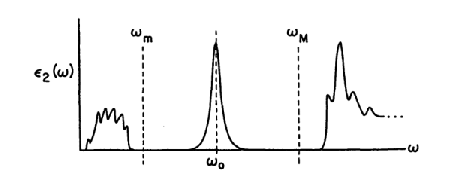
\includegraphics[width=8cm]{fig2.pdf}
\caption{Espectro de absorção de um material com uma linha de absorção estreita centrada na frequência $\omega_0$, bem separada da banda de absorção de frequências baixas, que pertencem à região $\omega < \omega_m$ e, também, bem separadas da banda de absorção de frequências altas que pertencem à região $\omega > \omega_M$.}
\end{figure}

A Eq. \eqref{eq37} descreve a variação de frequência de $\varepsilon_1(\omega)$ para $\omega$ próximo de uma linha isolada de absorção, \textbf{independente da origem física dessa absorção}. Se $\omega$ estiver próximo de $\omega_0$ mas ainda distante da linha de absorção, então $\varepsilon_2$ será muito pequeno e $\varepsilon(\omega)\approx\varepsilon_1(\omega)$. Antigamente, modelos mecânicos foram desenvolvidos para explicar a origem microscópica de expressões como a Eq. \eqref{eq37}. A motivação era o resultado experimental de que a parte real da função dielétrica, considerada como função da frequência, geralmente exibia um comportamento ressonante similar ao mostrado pela Eq. \eqref{eq37}. Para se obter o comportamento detalhado da distribuição de frequências da função dielétrica, é necessária a adoção de um modelo específico que possa ser calculado de maneira analítica. Um excelente modelo que é muito usado ainda hoje é o famoso modelo \textit{Lorentziano} do perfil de linha. O estudante poderá estudar as qualidades desse modelo através do exercício da lista de problemas. Iremos tratar nessa aula apenas materiais que possam ser descritos pela Eq. \eqref{eq37}.

\section{Propagação de uma Onda Eletromagnética num Meio Dispersivo}

O aluno demonstrará através da lista de exercícios que o campo eletromagnético satisfaz uma equação da onda. Soluções propagantes do tipo onda plana $\exp[i(\mathbf{k}\cdot\mathbf{r}-\omega t)]$ podem ser obtidas e no problema da lista de exercícios o aluno demonstrará que
\begin{equation}
    \frac{c^2 k^2}{\omega^2} = \varepsilon(\omega).
    \label{eq38}
\end{equation}
Suponha por um momento que a função dielétrica não depende da frequência. Então, a relação acima indica que a velocidade da frente de onda é constante
\begin{equation}
    v_{\text{p}} = \frac{\omega}{k} = \frac{c}{\sqrt{\varepsilon}}.
\end{equation}
A quantidade $\sqrt{\varepsilon}$ é portanto o índice de refração do material. Quando a função dielétrica depende da frequência, estamos interessados na função $\omega = \omega(k)$, chamada de \textbf{relação de disperção}. A relação de dispersão conecta os valores do vetor de onda $k$ com a frequência $\omega$ e caracteriza todas as propriedades de propagação da onda no meio. Utilizando a função dielétrica da Eq. \eqref{eq37}, é fácil demonstrar que
\begin{equation}
    \omega^{2}_{\pm}(k) = \frac{1}{2}\left( \frac{c^2 k^2}{\varepsilon_\infty} + \omega_0^2 + \frac{\Omega_p^2}{\varepsilon_\infty} \right) \pm \frac{1}{2}\sqrt{\left( \frac{c^2 k^2}{\varepsilon_\infty } + \omega_0^2 + \frac{\Omega_p^2}{\varepsilon_\infty} \right)^{2} - 4\omega_0^2 \frac{c^2 k^2}{\varepsilon_\infty}}.
\end{equation}
Existem portanto duas bandas de frequência, uma abaixo de $\omega_0$ e a outra acima de $\sqrt{\varepsilon_s/\varepsilon_\infty}\omega_0$, onde $\varepsilon_s = \varepsilon_\infty + \Omega_p^2 /\omega_0^2$. Na região de frequências entre esses dois valores, $\varepsilon$ é negativo e, de acordo com a Eq. \eqref{eq38}, o vetor de onda deve ser imaginário o que implica uma onda evanescente que não se propaga dentro do material.

\begin{figure}[ht]
\centering
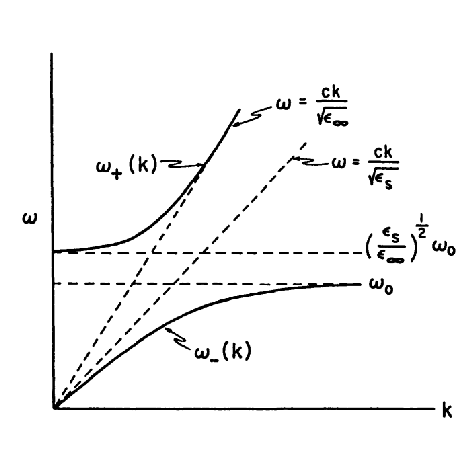
\includegraphics[width=8cm]{fig3.pdf}
\caption{A relação de dispersão para ondas eletromagnéticas que se propagam num meio com uma função dielétrica descrita pela Eq. \eqref{eq37}. A quantidade $\varepsilon_s$ é a constante dielétrica estática $\varepsilon_s = \varepsilon_\infty + \Omega_p^2 /\omega_0^2$.}
\end{figure}

\section{Natureza Física da Banda de Absorção Eletrônica}

Qual a natureza física da ressonância descrita pela função dielétrica? Como a forma da função $\varepsilon_2 (\omega)$, que está relacionada à absorção de energia do campo para o meio, pode ser explicada de um ponto de vista mais fundamental? A forma de $\varepsilon(\omega)$ mostrada na Eq. \eqref{eq37} se aplica a qualquer substância na qual encontra-se uma banda de absorção estreita separada em frequência de outras bandas. Essa descrição pode ser aplicada em gases, por exemplo. Num gás, as moléculas estão bem separadas uma das outras, de modo que a energia do sistema consiste em várias bandas estreitas de absorção. Cada nível de energia tem degenerescência $N$, onde $N$ é o número total de átomos no gás. Na matéria condensada, como um sólido ou líquido, as funções de onda dos elementos constituintes se sobrepõem e o espectro de absorção é um pouco mais complexo do que o espectro de um gás (que consiste de várias linhas estreitas uma das outras). Cada nível de energia com degenerescência $N$ evolui para uma banda contendo $N$ níveis muito próximos uns dos outros, como ilustra a Fig. 4. assim, esperamos que a forma da função $\varepsilon_2 (\omega)$ para um gás consista de vários picos extremamente estreitos enquanto que a forma da mesma função para um sólido ou líquido consista de vários picos com uma largura maior, já que existem mais energias disponíveis para o elétron fazer uma transição eletrônica.

\begin{figure}[ht]
\centering
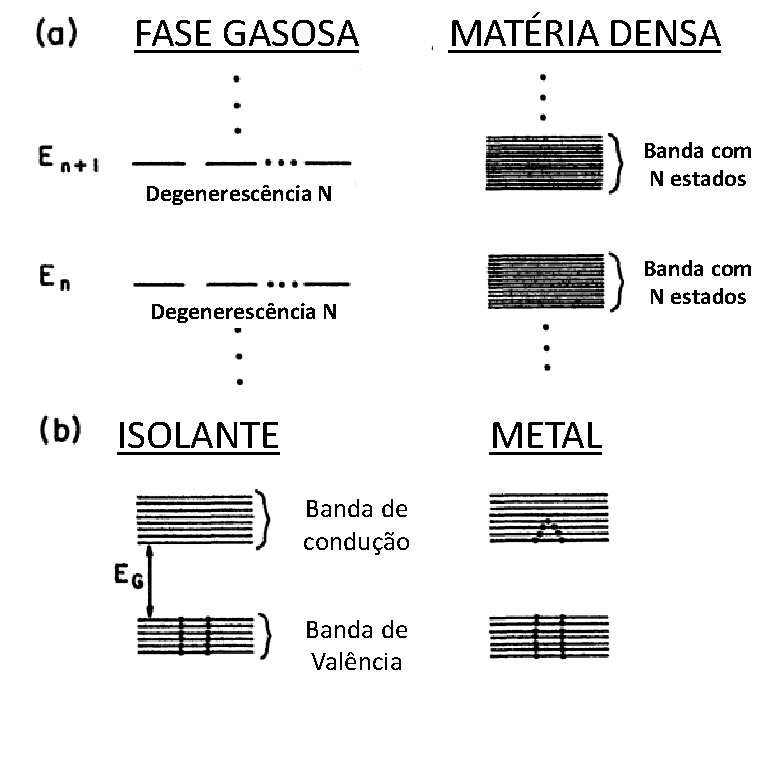
\includegraphics[width=8cm]{fig4.pdf}
\caption{(a) O espectro dos níveis de energia é ilustrado de forma esquemática para uma coleção de $N$ átomos num gás e para uma coleção na fase densa, como um sólido ou líquido. (b) Ilustração da ocupação dos elétrons num isolante e num metal.}
\end{figure}

Além disso, podemos classificar a grande classe de materiais em dois tipos: isolantes e condutores. Isolantes não carregam uma corrente elétrica quando colocados em contato com um campo elétrico estático enquanto que os condutores geram uma corrente. As propriedades de qualquer material são controladas pela maneira na qual os elétrons estão distribuídos nos níveis de energia do material. O princípio da exclusão de Pauli diz que apenas dois elétrons podem ser colocados em cada estado, um com spin ``para cima'' e outro com spin ``para baixo''. Se cada átomo contém um número par de elétrons, então uma simples contagem mostra que irão preencher os primeiros $n/2$ níveis de energia, onde $n$ é o número de elétrons por átomo. Essa situação está ilustrada na parte da esquerda da Fig. 4 (b). O primeiro estado excitado está a uma distância $E_g$ acima da banda de energia ocupada, chamada de banda de valência. A energia $E_g$ é chamada de \textit{bandgap}. Para promover um elétron da banda de valência para a \textit{banda de condução} é necessário absorver uma energia mínima de $E_g$. A banda de condução tem esse nome porque elétrons que estão nessa banda são movidos pelo material quando um campo elétrico estático está presente. Para um número ímpar de elétrons por átomo, a banda mais alta de energia está parcialmente ocupada, como ilustra o painel à direita na Fig. 4. Nesse caso, um campo elétrico estático induz movimento de cargas e, consequentemente, a criação de uma corrente elétrica. Materiais que possuem um essa característica são chamados condutores.

Um outro aspecto de ressonâncias eletrônicas (isto é, que levam em conta apenas transições de estados eletrônicos e não vibracionais, por exemplo), está relacionado aos chamados éxcitons. Quando um elétron é promovido da banda de valência para a banda de condução, após receber uma certa energia maior ou igual ao bandgap, o mesmo deixa um buraco na banda de valência. O buraco possui uma carga positiva e é atraído pelo elétron que deixou a banda por conta da lei de Coulomb. Essa entidade formada pela atração Coloumbiana entre o buraco e o elétron é chamada de éxciton. O interessante nesse fenômeno é que a energia de atração (ou, em outras palavras, a energia para a formação do éxciton) é um pouco menor que a energia do bandgap $E_g$. Dessa forma, num espectro de absorção, um pouco antes da borda da absorção, ocorrem picos discretos de energia. 

\section{Conclusão}

Tratamos nessa aula a resposta eletromagnética da matéria de um ponto de vista macroscópico descrito pelas equações de Maxwell. Claramente, o tema é muito complexo e não foi mencionamos sequer outros tipos de contribuições que podem aparecer na interação radiação-matéria. Os modos vibracionais das moléculas ou dos átomos em torno de suas posições de equilíbrio (chamados fônons) desempenham um papel importantíssimo na descrição do acoplamento da luz com o movimento mecânicao da rede (acoplamento fóton-fônon) e o aluno que quiser se aprofundar nesses temas pode procurar as referências citadas no plano de aula.













\end{document}
